%--------------------------------------------------------------------------------------------
%   YART thesis "YART: A Ray Tracing Application" chapter definition.
%--------------------------------------------------------------------------------------------

\chapter{YART: A Ray Tracing Application} \label{ch:Application}
\vspace*{-2pt}

Proposed by this dissertation, \textit{Yet Another Ray Tracer} (YART) is a cross-platform 3D rendering application with an integrated ray tracing engine. 
It was build using the C++ programming language with a goal of exploring the inner workings of a ray tracing system and testing the capabilities of modern hardware.
The rendering engine has been entirely prepared on the CPU, using a traditional, object oriented approach.
As opposed to many state-of-the-art renderers which focus greatly on high performance and efficiency, YART is instead designed to be an easily customizable and scalable environment. 
While not prioritizing the engines performance, treading is used in various parts of the system to utilize the power of CPU parallelization.
In parts not directly related to ray tracing, the application's backend makes use of GPU capabilities for creating a window, and presenting subsequent frames onto it.
Additionally, YART aims to be highly interactive and verbose.
The application's graphical user interface (GUI) is designed to enable easy access to various parts of the engine, otherwise not exposed in similar, commercial software. 
YART's source code can be found in the project's official GitHub repository: \url{https://github.com/hhimko/yart}. 

\section{Application Architecture}

YART's architecture can be divided into two key components.
The first of which, further referred to as the \textit{backend}, is dedicated to performing lower-level operations, such as opening and managing the application window, polling incoming inputs, as well as displaying application frames. 
It aims to abstract away platform-dependant functionalities, with the use of a lightweight API, designed to be implemented using various windowing systems and libraries. 
In general, the backend encapsulates every system-agnostic feature within YART, which could be related to GPU programming.

Everything beyond the backend, can be collectively referred to as the \textit{application core}. 
As the name implies, it consists of key application modules, which primarily include the ray tracing engine and the user interface.
The renderer does not directly depend on its system's backend, and vice versa. 
It has been designed to write its pixel output into an ordinary C-style array, not caring what happens to it afterwards.
Using this methodology, enables the renderer to be easily reused in various parts of the application, such as for rendering material preview viewports within the UI.

The backend and the application core are separated with the aim of decoupling system- and hardware-agnostic functionality from the rendering engine.
What binds them together, is a central \verb|yart::Application| class, designated to initializing both components and communicating between them using specialized callbacks. 
Furthermore, it introduces the \textit{mainloop}, which defines the fundamental control flow of every application frame.
The YART application architecture, with its components and relations made between them, is illustrated in \cref{fig:Application/ApplicationArchitecture/arch}. 

\begin{figure}[!ht]
    \centering
    \vspace*{3mm}

    \newcommand{\arrowshift}{95pt}

    \begin{tikzpicture}[auto]
        % Application core inner modules
        \node[module] (engine) {Ray Tracing Engine};
        \node[module, right=5mm of engine] (gui) {User Interface (UI)};

        \draw[->, thick] (gui) to (engine);

        % Application core label
        \node[draw=none, fit=(engine) (gui)] (core-modules) {};
        \node[font=\large, above=-1mm of core-modules, inner sep=4pt] (core-label) {Application Core};

        % Application core component
        \begin{pgfonlayer}{background}
            \node[component, fit=(core-modules) (core-label), minimum width=10cm] (core) {};
        \end{pgfonlayer}

        % Application class 
        \node[draw, rounded corners, inner sep=6pt, font=\bfseries\small, below=14mm of core, minimum width=97mm] (mainloop) {mainloop};
        \node[font=\large, above=0mm of mainloop, inner sep=4pt] (application-label) {\verb|yart::Application| Class};

        \begin{pgfonlayer}{background}
            \node[main, thick, fill=blue!5, fit=(mainloop) (application-label)] (application) {};
        \end{pgfonlayer}
        \draw[->, thick] ([xshift=\arrowshift]application.north west) to ([xshift=\arrowshift]core.south west);
        \draw[->, thick] ([xshift=-\arrowshift]core.south east) to ([xshift=-\arrowshift]application.north east);

        % Backend component
        \node[component, below=5mm of application] (backend) {Backend};
        \draw[<-, thick] ([xshift=\arrowshift]application.south west) to ([xshift=\arrowshift]backend.north west);
        \draw[<-, thick] ([xshift=-\arrowshift]backend.north east) to ([xshift=-\arrowshift]application.south east);
    \end{tikzpicture}

    \caption[YART application architecture]{YART application architecture.}
    \label{fig:Application/ApplicationArchitecture/arch}
\end{figure}

Introduction of the \verb|yart::Application| class implies, that the engine can be detached from the windowing backend, and easily transformed into other application types.
For example, the YART engine could be reused as an offline renderer within a new console application, or used as a ray tracing library in already existing systems.

\section{Functionality Overview}

YART allows for rendering complex, user-defined scenes, which are mainly composed of mesh geometry, light sources and a customizable environment.
The application's UI introduces a set of tools and functionalities, which provide the end user with the ability to manage a scene, and customize various parts of the rendering engine.
Users can open new and empty scenes, and populate them with numerous primitives, such as cubes, spheres or planes.
Alternatively, a number of example scenes can be loaded via the application's main menu bar, and tailored depending on personal needs. 
The object hierarchy window displays all created scene objects and their individual properties, enabling further edition.
Objects selected in the hierarchy view can be freely translated and rescaled, allowing for a high variety of custom scenes.
Additionally, every object defines its own, customizable material, which influences its appearance and reflectance properties.
To avoid rendering scenes inside a black void, skies can be shaded using three methods employed in the engine: solid color skies, linear gradient skies, and textured skyboxes.
\cref{fig:Application/FunctionalityOverview/render_sample} illustrates a sample scene, rendered using the YART application's ray tracing engine.

\begin{figure}[!ht]
    \centering
    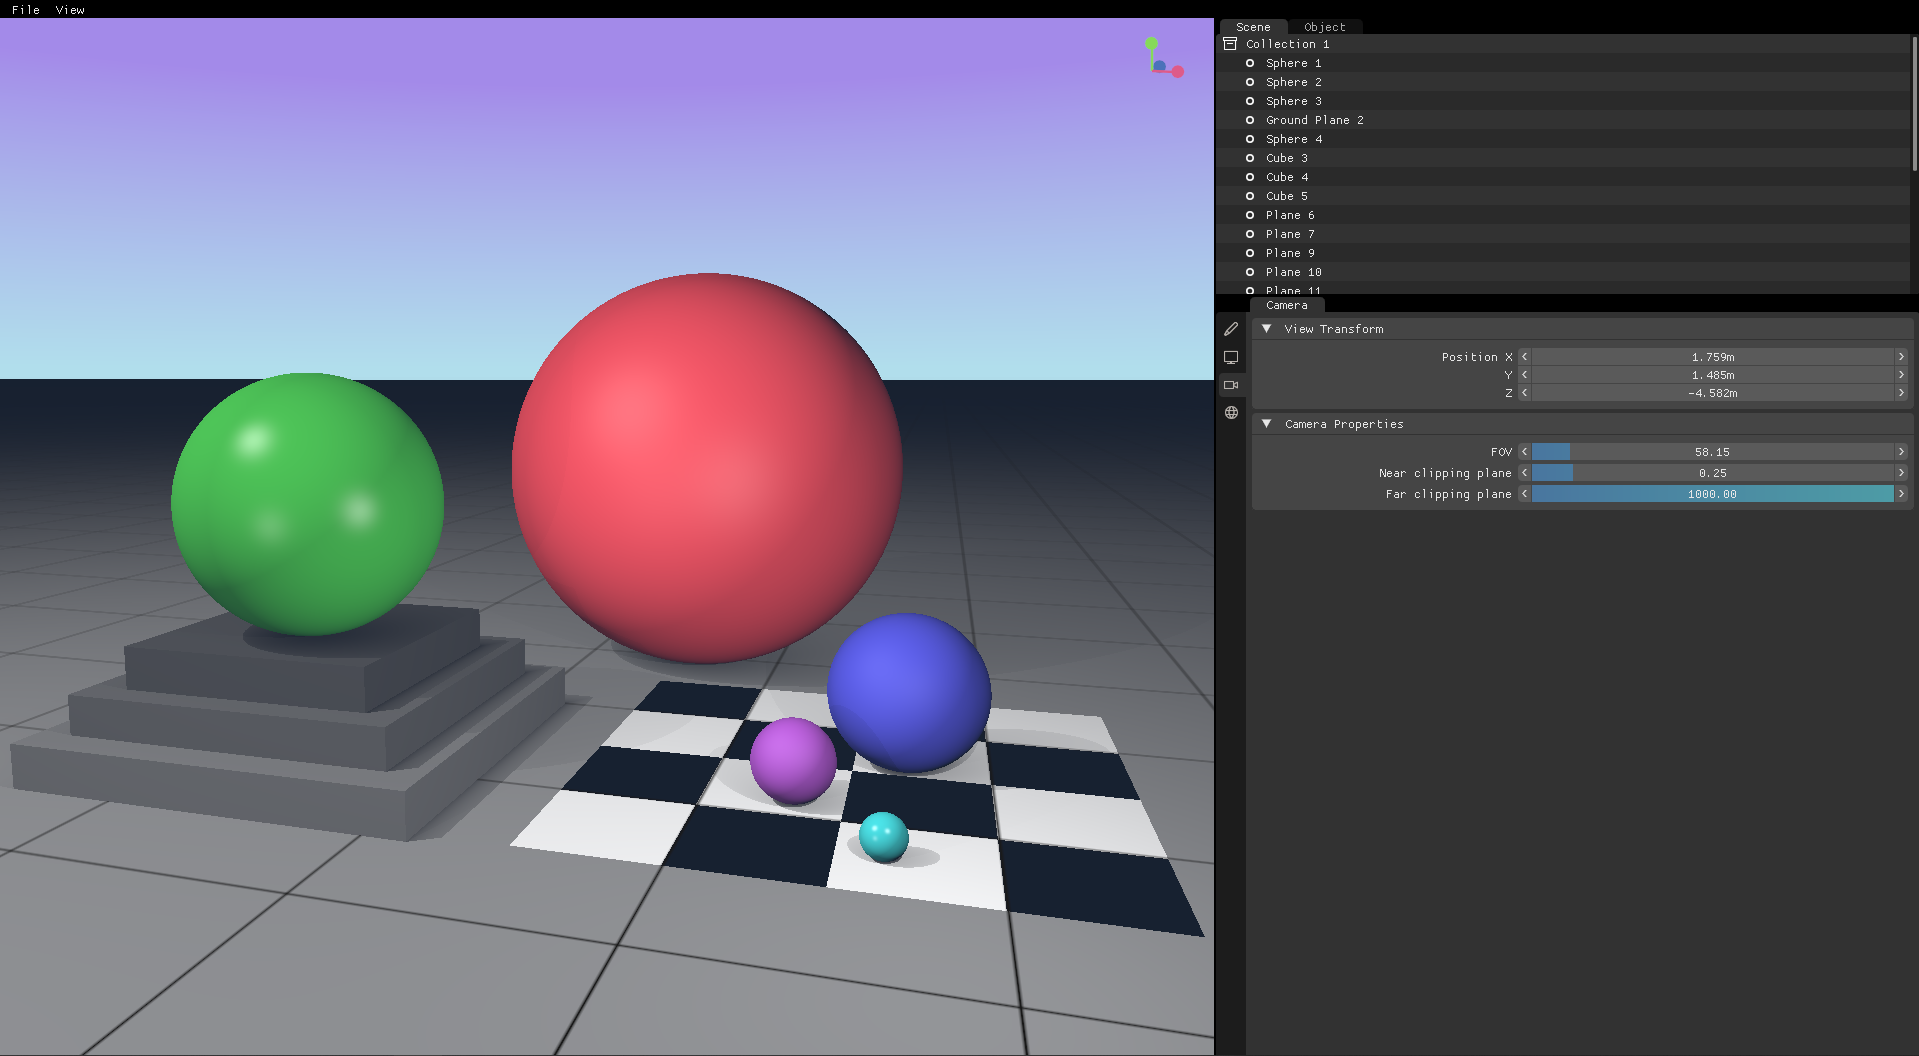
\includegraphics[height=8cm]{res/SampleRender.png}
    \caption[Example image rendered using the YART engine]{Example image rendered using the YART engine.}
    \label{fig:Application/FunctionalityOverview/render_sample}
\end{figure}

\section{External Dependencies}

All dependencies excluding Vulkan are included into, and built with the project, in the form of \textit{Git submodules}. 
Incorporated into the distributed version control system -- Git, submodules provide functionality to include separate Git repositories as subdirectories within another project.
The only closed-source dependency used within the project, is the Vulkan library.
In order for the application to build, the Vulkan software development kit (SDK) has to be installed on the users machine. 
Following, is a list of all external dependencies used throughout the YART application, including a brief description and their purpose within the project.

\subsection{GLFW}

GLFW \supercite{GLFW} is a lightweight C library for creating and managing windows.
It provides a multi-platform abstraction layer, primarily designed to work seamlessly with applications made using OpenGL \supercite{Neider1993}.
The GLFW API includes a straightforward mechanism for handing inputs such as keyboard or mouse, as well as various time management functions, making it easier to control the frame rate of an application.
YART makes use of GLFW to open a platform-specific window and handle all incoming user inputs. 
The window is used as a rendering surface, to which the GPU can draw subsequent application frames. 
GLFW exposes user input in the form of events, which can be polled and handled using specific callbacks. 
The event system is utilized within YART to handle key presses and mouse events for various interactions, such as viewing-camera movement and rotation.

\subsection{Vulkan}

Developed by the Khronos Group, Vulkan \supercite{Sellers2016} is a low-level graphics and compute programming interface.
Designed as a successor to the prominent OpenGL API, it provides an efficient and flexible framework for graphics programming on modern GPUs.
Unlike some higher-level graphics libraries, Vulkan does not hide, or abstract away the underlying hardware details or perform certain optimizations automatically. 
Instead, developers are equipped with high degree of control and responsibility.
Memory, synchronization, and devices have to be managed explicitly, leading to increased verbosity in the code.
Proper use of Vulkan capabilities can lead to better utilization of system resources and improved performance in graphics-intensive applications.

Vulkan, along with GLFW, serves as the window rendering backend for the YART application.
It does not however play any role in performing actual ray tracing computations, which are made entirely on the CPU. 
Instead, the backend utilizes the pixel output of the engine's renderer, which gets streamed into a texture and displayed every frame within a viewport.
For this purpose, a specialized graphics pipeline is deployed using Vulkan, that in its core, issues render commands to the GPU and presents frames to the GLFW window. The pipeline was designed to adapt to a high variety of hardware devices, taking advantage of their characteristics.
For example, depending on the capabilities of a physical device installed on the client's machine, multiple frames can be prepared in parallel, which can greatly improve the application's performance.
Querying these capabilities, allows the backend to optimize its render pipeline, and to target the most applicable device, in scenarios where multiple GPUs are available.

\subsection{Dear ImGui}

Dear ImGui \supercite{DearImGui}, is a versatile, open-source graphical user interface (GUI) library for the C++ language. 
It is fast, portable, and comes with a variety of UI components, that can easily be customized and styled.
ImGui is primarily designed as an interactive debugging tool for use in real-time rendering applications, video games, or other environments where GUI creation features are non-standard.
YART however, extends on Dear ImGui's standard feature set, to define custom widgets and render the final user interface layout. 
At its core, Dear ImGui is what makes the application interactive, enabling the end user to tinker with the engine's functionality.

\subsection{GLM}

OpenGL Mathematics (GLM \supercite{GLM}), is a C++ mathematics library designed specifically for graphics programming and game development.
It is lightweight, self contained, and header-only, meaning it does not use any external dependencies, and does not need to be separately compiled or linked.
YART benefits from vector and matrix operations available in GLM, which are essential for various rendering tasks, such as defining projections and calculating transformations.
